\documentclass{beamer}
\usetheme[progressbar=frametitle]{metropolis}          % Use metropolis theme

\graphicspath{{../src/images/}}

\usepackage{longtable}
\usepackage{pdfpages}	


% change progressbar thickness
\makeatletter
\setlength{\metropolis@titleseparator@linewidth}{1.5pt}
\setlength{\metropolis@progressonsectionpage@linewidth}{1.5pt}
\setlength{\metropolis@progressinheadfoot@linewidth}{2pt}
\makeatother

\usepackage{FiraSans}
\usepackage{makecell}
\usepackage{appendixnumberbeamer}

\title{Bezdrátová senzorová síť pro přístupový systém}
\date{25.6.2020}
\author{Bc. Tomáš Hyhlík}
\institute{Diplomová práce}
\begin{document}
  \maketitle

  

  %%%%%%%%%%%%%%%%%%%%%%%%%%%%
	\begin{frame}{Integrace WSN do architektury přístupového systému}

		\begin{figure}[h]
			\centering
			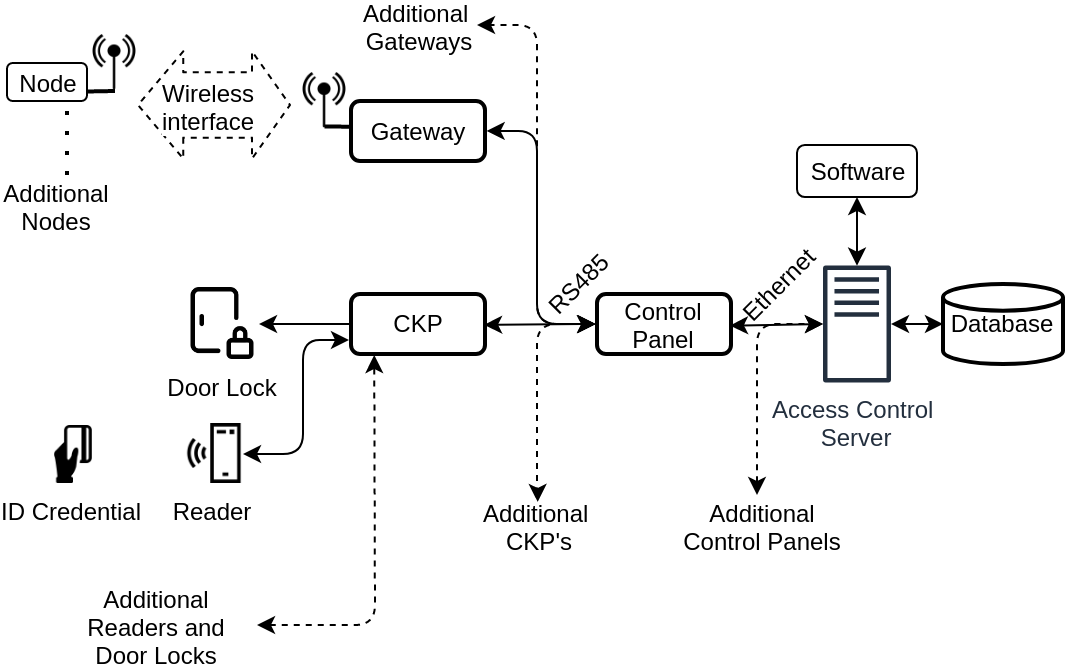
\includegraphics[width=1\textwidth]{ACS_IoT_extension_21}
			% \caption{Architektura přístupového systému firmy IMA s rozšířením o gateway senzorové sítě}
			\label{fig:ACS architecture IMA with geteway}
		\end{figure}
			
	\end{frame}









  %%%%%%%%%%%%%%%%%%%%%%%%%%%%
  \begin{frame}{Výběr bezdrátové technologie}

	Požadavky:
	\begin{itemize}
		\item Nízká cena HW
		\item Jednoduché přípojení koncových zařízení třetích stran (Third party)
		\item Velký počet dostupných koncových zařízení třetích stran na trhu 
		\item Jednoduchá implementace
		\item Nízká spotřeba energie koncových zařízení
	  \end{itemize}

  \end{frame}


  %%%%%%%%%%%%%%%%%%%%%%%%%%%%
  \begin{frame} {WSN gateway - HW}
	  
	\begin{figure}[!h]
		\centering
		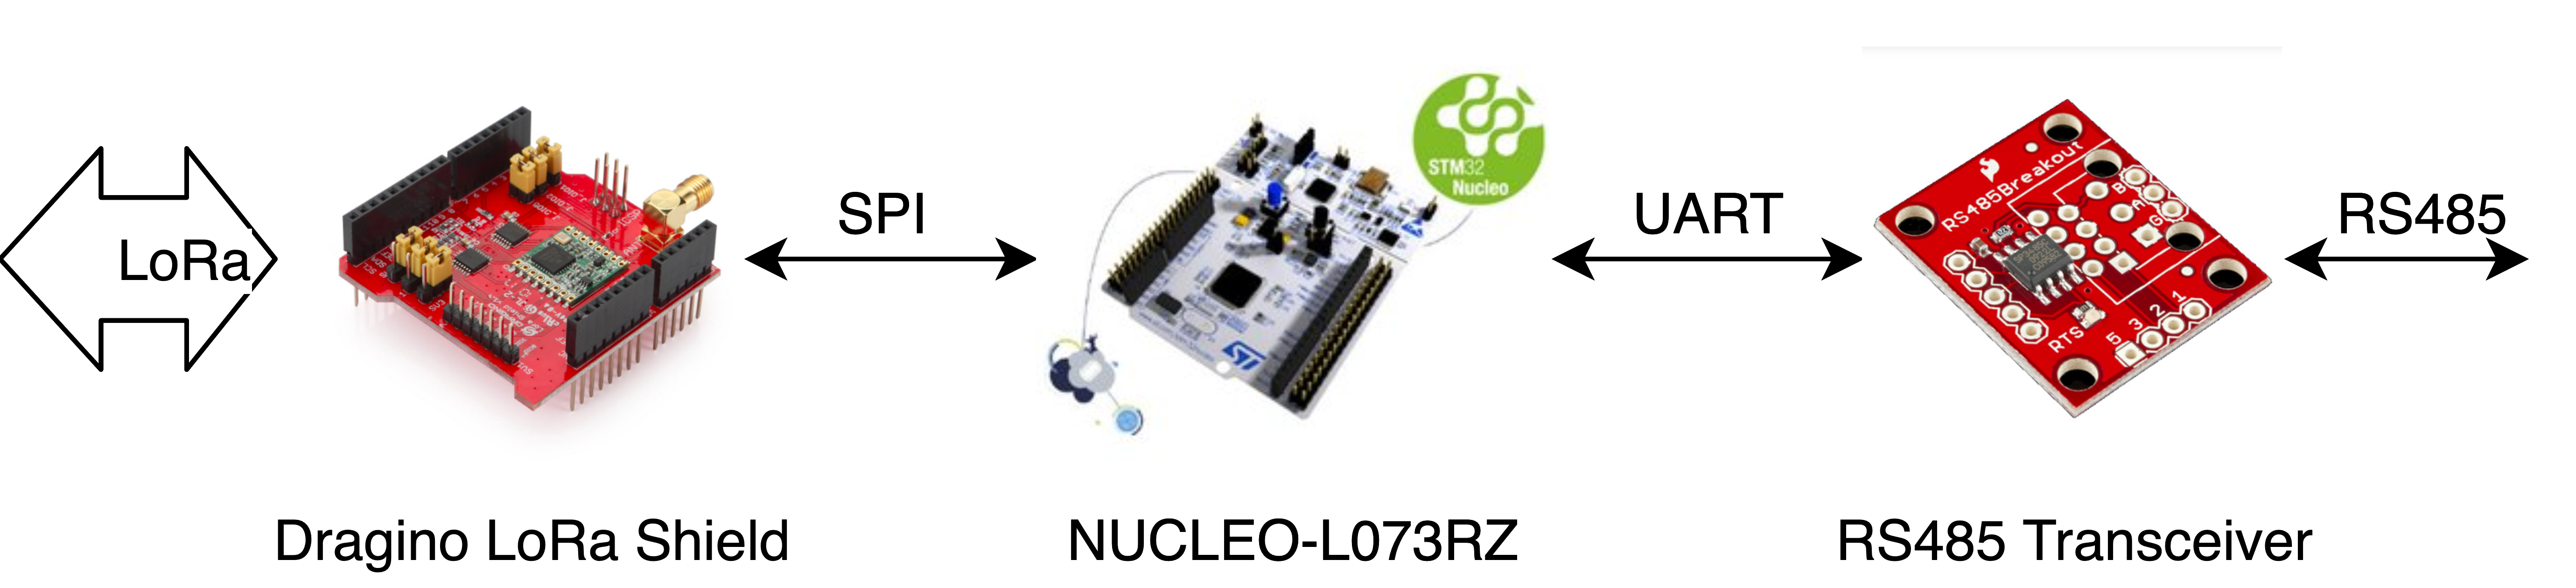
\includegraphics[width=1\textwidth]{LoRaWAN_gw_RS485_blockDiagram_3}
		% \caption{Blokový diagram navržené gatewaye senzorové sítě, Dragino LoRa Shield \cite{draginoWiki}, RS485 transceiver \cite{rs485tr}, NUCLEO-L073RZ \cite{nucleo-l073RZ_ST}}
		\label{fig:gatewayBlockDiagram}
	\end{figure}

  \end{frame}

  %%%%%%%%%%%%%%%%%%%%%%%%%%%%
  \begin{frame} {WSN gateway - SW bloky}

	{\fontsize{10}{6}\selectfont 

	\begin{longtable}{ |l|p{7cm}| }
		% \caption{Rozdělení programu na nezávislé podprogramy}
		% \label{table:sw_div} \\
		\hline
		% Název podprogramu  & Popis           \\ \hline \hline
		LoRa            &  Knihovna zahrnující komunikaci s transceiverem RFM95W po rozhraní SPI, nainicializovaném v režimu komunikace LoRa    \\ \hline
		LoRaWAN\_packet  & Knihovna zahrnující LoRaWAN protokol, tedy dekódování a dešifrování přijatého LoraWAN paketu i vytvoření paketu pro odeslání. Tato knihovna je závislá na knihovnách aes a cmac.  \\ \hline
		LoRa\_sensors    & Knihovna zahrnující dekódování payloadu podporovaných koncových zařízení a zapsání výsledných hodnot do bufferu, který je pak odeslán na kontrolní panel přes síť RS485       \\ \hline
		rs485\_protocol  & Podprogram zahrnující síťový protokol v síti RS485         \\ \hline
		usb             &  Podprogram zahrnující konfiguraci systému přes USB        \\ \hline
		eeprom          &  Knihovna zahrnující práci s non-volatile paměti procesoru EEPROM     \\ \hline

	\end{longtable}
	}

\end{frame}


  %%%%%%%%%%%%%%%%%%%%%%%%%%%%
  \begin{frame} {WSN gateway - SW}

	{\fontsize{5}{6}\selectfont 
	
	
	
	
	}


  \end{frame}



  %%%%%%%%%%%%%%%%%%%%%%%%%%%%
  \begin{frame} {WSN gateway - SW}



  \end{frame}



%   \appendix
%   \begin{frame}{Reference}
  	
%   	 \bibliography{aeda_prezentace_bib}
% 	 \bibliographystyle{abbrv}
  	
%   \end{frame}

\end{document}